\documentclass{article}
\usepackage{titling}
\usepackage[T1]{fontenc}
\usepackage[polish]{babel}
\usepackage[OT4]{fontenc} 
% Margins in document
\usepackage[left=1.5cm, right=1.5cm, top=3cm]{geometry}

% Avoid  colons before tables' empty captions and change caption
\usepackage{caption}
\captionsetup[table]{name=Tab.}
\captionsetup[figure]{name=Rys.}
\usepackage{hyperref}

% Don't know why, it starts from 2
\addtocounter{table}{-1}

% Rename tables' suffix
\renewcommand{\tablename}{Tab.}

% Graphicx setup
\usepackage{graphicx}
\graphicspath{{grafiki/}{../grafiki/}}

% No separator between items
\usepackage{enumitem}
\setlist{nolistsep}

% Pagebreak before every \section
\let\oldsection\section
\renewcommand\section{\clearpage\oldsection}

% Vhistory setup
\usepackage[owncaptions]{vhistory}
\renewcommand{\vhhistoryname}{Historia zmian}
\renewcommand{\vhversionname}{Wersja}
\renewcommand{\vhdatename}{Data}
\renewcommand{\vhauthorname}{Autor(zy)}
\renewcommand{\vhchangename}{Zmiany}

% Bigger padding in tabulars
\usepackage{array}
\setlength\extrarowheight{3pt}

% Itemize in tabulars (avoid big margins with minipage)
\newcommand{\tabbeditemize}[1]{
	\begin{minipage}[t]{0.4\textwidth}
		\begin{itemize}[topsep=0mm,partopsep=0mm,leftmargin=4mm]
			#1
		\end{itemize}
\end{minipage}}

% Code command
\usepackage{xcolor}
\definecolor{light-gray}{gray}{1}
\newcommand{\code}[1]{\colorbox{light-gray}{\texttt{#1}}}

% Modulename command
\newcommand{\modulename}[1]{\textit{#1}}

% Listings setup
\usepackage{listings}
\definecolor{codegreen}{rgb}{0,0.6,0}
\definecolor{codegray}{rgb}{0.5,0.5,0.5}
\definecolor{codepurple}{rgb}{0.58,0,0.82}
\definecolor{backcolour}{rgb}{0.95,0.95,0.92}
\lstdefinestyle{mystyle}{
	backgroundcolor=\color{backcolour},   
	commentstyle=\color{codegreen},
	keywordstyle=\color{magenta},
	numberstyle=\tiny\color{codegray},
	stringstyle=\color{codepurple},
	basicstyle=\ttfamily\footnotesize,
	breakatwhitespace=false,         
	breaklines=true,                 
	captionpos=b,                    
	keepspaces=true,                 
	numbers=left,                    
	numbersep=5pt,                  
	showspaces=false,                
	showstringspaces=false,
	showtabs=false,                  
	tabsize=2
}
\lstset{style=mystyle}

% DOCUMENT
\title{
	Wizualizacja drzewa stanów algorytmu UCT \\
	\large Dokumentacja powykonawcza}

\author{Patryk Fijałkowski \\ Grzegorz Kacprowicz}
\begin{document}
\begin{titlingpage}
	\maketitle
	\vspace{3cm}
	\begin{abstract}
		Poniższy dokument zawiera dokumentację powykonawczą projektu, którym było stworzenie aplikacji pozwalającej na wizualizację drzewa stanów algorytmu UCT. Ma ona w zamyśle pozwalać na oglądanie i dokładną analizę rozgrywki z komputerem podczas grania w jedną z dwóch gier planszowych. Dokument przeprowadza czytelnika przez instrukcję poprawnego uruchomienia programu oraz opis funkcjonalności połączony z instrukcją użytkowania. Będzie on zawierał również opis interfejsu użytkownika, dokładnie opisujący najistotniejsze okna aplikacji. Dokument pozwala także zaznajomić się z architekturą programu oraz opisem i schematami modułów aplikacji - zaczynając od tego odpowiedzialnego za wizualizację. Pierwszy moduł, będący najistotniejszym, będzie opierał się na usprawnionej wersji algorytmu Walkera. Opisane są również moduły odpowiedzialne za logikę zaimplementowanych gier, implementację algorytmu oraz serializowanie generowanych drzew wraz ze schematami serializacji. \modulename{Aplikacja główna}, czyli ostatni opisywany moduł, jest modułem służącym do prezentacji działania poprzednich modułów. Ostatni rozdział dokumentu opisuje i uzasadnia technologie wybrane do stworzenia aplikacji.
	\end{abstract}
\end{titlingpage}

\begin{versionhistory}
	\vhEntry{1.0}{10.12.2019}{PF|GK}{stworzenie szkicu dokumentu}
\end{versionhistory}
\tableofcontents
	
\section{Instrukcja uruchamiania}
Aplikacja została napisana w języku \textit{Python}, zatem klient powinien zainstalować jego interpreter, który może znaleźć na stronie: \url{https://www.python.org/downloads/}. Wymagana wersja to Python 3.7.2 lub nowsza.\\
Do tak ściągniętego interpretera załączony jest również \textit{pip} - menedżer pakietów Python. Za jego pomocą należy pobrać niezbędny pakiet. Przed pobraniem pakietów zalecane jest uaktualnienie menedżera następującą komendą:
\begin{itemize}
	\item na Windowsie:
	\begin{lstlisting}
	python -m pip install -U pip\end{lstlisting}
	\item na Linuxie:
	\begin{lstlisting}
	pip install -U pip\end{lstlisting}
\end{itemize}
Następnie, należy uruchomić następującą komendę w konsoli, aby pobrać pakiet PyQt5, o którym więcej będzie w ostatnim rozdziale dokumentu:
\begin{lstlisting}
pip install PyQt5
\end{lstlisting}
Ze względu na fakt, iż Python jest językiem interpretowanym, program również należy uruchomić \underline{z poziomu konsoli}. 
Należy zatem przejść do katalogu \textbf{/uct-visualization/src/main\_application} i wpisać komendę:
\begin{lstlisting}
python main_application_window.py
\end{lstlisting}
lub uruchomić program z głównego katalogu aplikacji \textbf{/uct-visualization}:
\begin{lstlisting}
python /uct-visualization/src/main_application/main_application_window.py
\end{lstlisting}
Po uruchomieniu powinniśmy zobaczyć główne okno aplikacji o nazwie \textit{UCT Visualizer}.

\section{Poradnik użytkowania}
\subsection{Okno główne aplikacji}
\begin{center}
	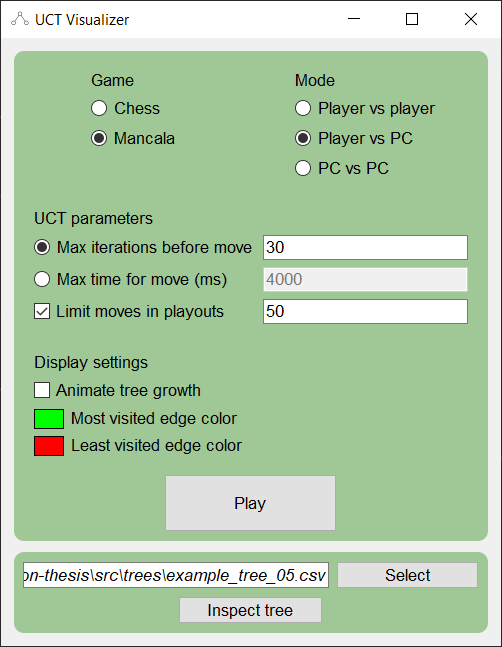
\includegraphics[width=0.6\textwidth]{main-app-window}
\end{center}
\subsection{Okno podglądu drzewa}
\begin{center}
	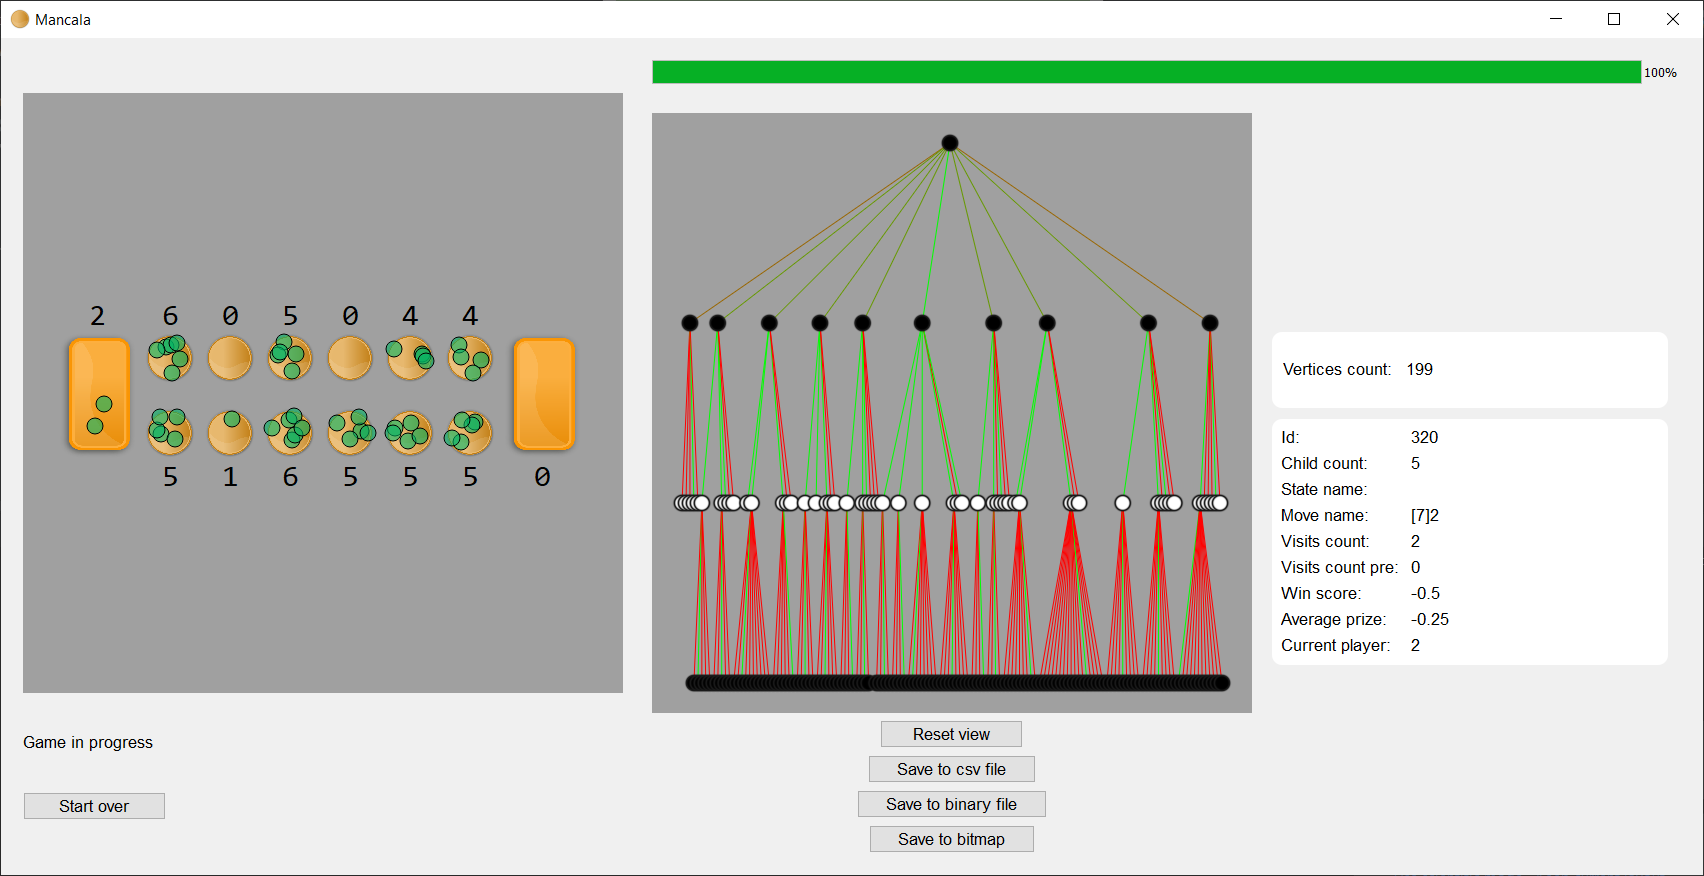
\includegraphics[width=1\textwidth]{game-window}
\end{center}
\subsection{Okno gry i wizualizacji}
\begin{center}
	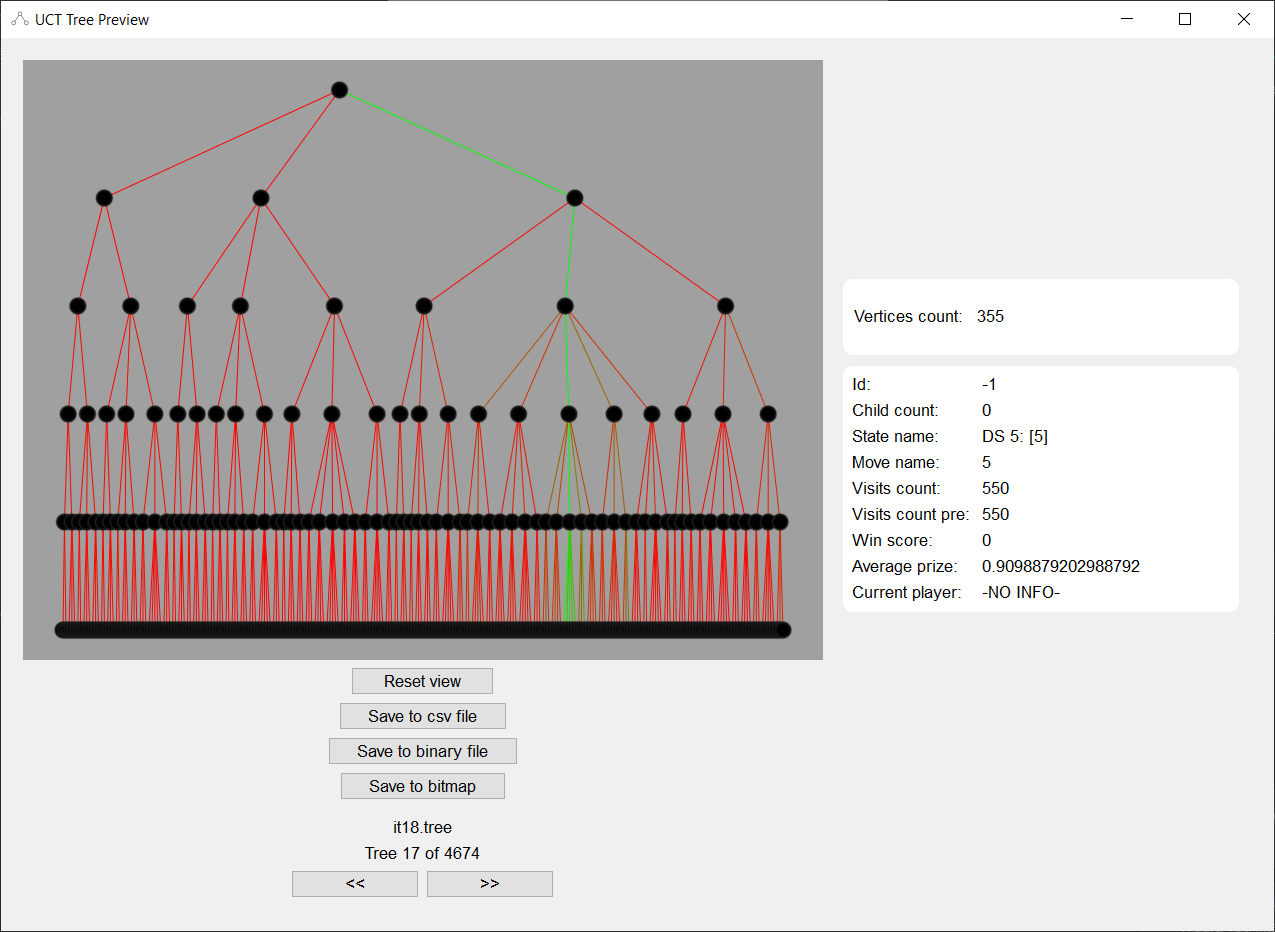
\includegraphics[width=1\textwidth]{tree-window}
\end{center}

\section{Architektura systemu}
\section{Użyte technologie}
\end{document}
